\documentclass[a4paper,10pt]{article}
%\usepackage[utf8x]{inputenc}
%\usepackage{czech}
\usepackage[utf8]{inputenc}
\usepackage[czech]{babel}
\usepackage{graphicx}
\usepackage{subfig}

\title{Zpráva k~seminární úloze z~předmětu\\ Inteligentní robotika \\ {\small Závěrečná zpráva}}
\author{Filip Jareš, Lenka Mudrová}
\date{27.4.2011}

\begin{document}

\maketitle
\begin{figure}[!h]
	\centering
	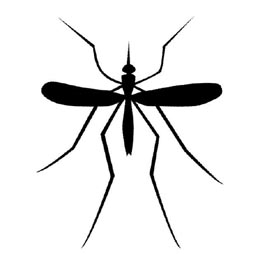
\includegraphics[width=0.4\columnwidth]{pics/mosquito}
	%\caption{}\label{fig:m}
\end{figure}
\newpage

\section{Popis úlohy}
		Řešená úloha je inspirována článkem Backyard star wars \cite{zadani}, který se zabývá problémem
		detekce komára ve venkovním prostředí a jeho sestřelení laserovým paprskem. 
		Pro školní účely byla tato myšlenka pozměněna, komár je nahrazen černým čtvercem, který se pohybuje na bílém
		pozadí monitoru, namísto laseru je pouze sledován kamerou.

		Poloha kamery se ovládá s použitím dvou modelářských serv a to  
		natočením okolo svislé osy (změnou azimutu) a natočením okolo vodorovné osy (změnou elevace). Cílem úlohy
		je řídit kameru tak, aby sledovala pohyb komára a zdokumentovala jeho „sestřel“
		sérií snímků, ve kterých je komár ve středu obrazu z~kamery – uprostřed
		„záměrného kříže“.

		

\section{Rozbor problému}
		Úloha se skládá z~několika oblastí, především je zde zastoupena oblast
		po\-čí\-ta\-čo\-vé\-ho vidění, kdy je nutné sejmout obrázek z~kamery, zpracovat ho a
		detekovat v~obraze komára. 
		Další oblastí, která je zastoupena, je řízení. K zaměření a „sestřelu“ komára je
		třeba regulovat pohyb kamery.
		V~neposlední řadě je v~problému zastoupena robotika, kdy je potřeba pracovat se
		soustavou serv a počítat transformace souřadnic mezi obrazovkou a souřadným
		systémem serv.

		\begin{figure}[!h]
			\centering
			 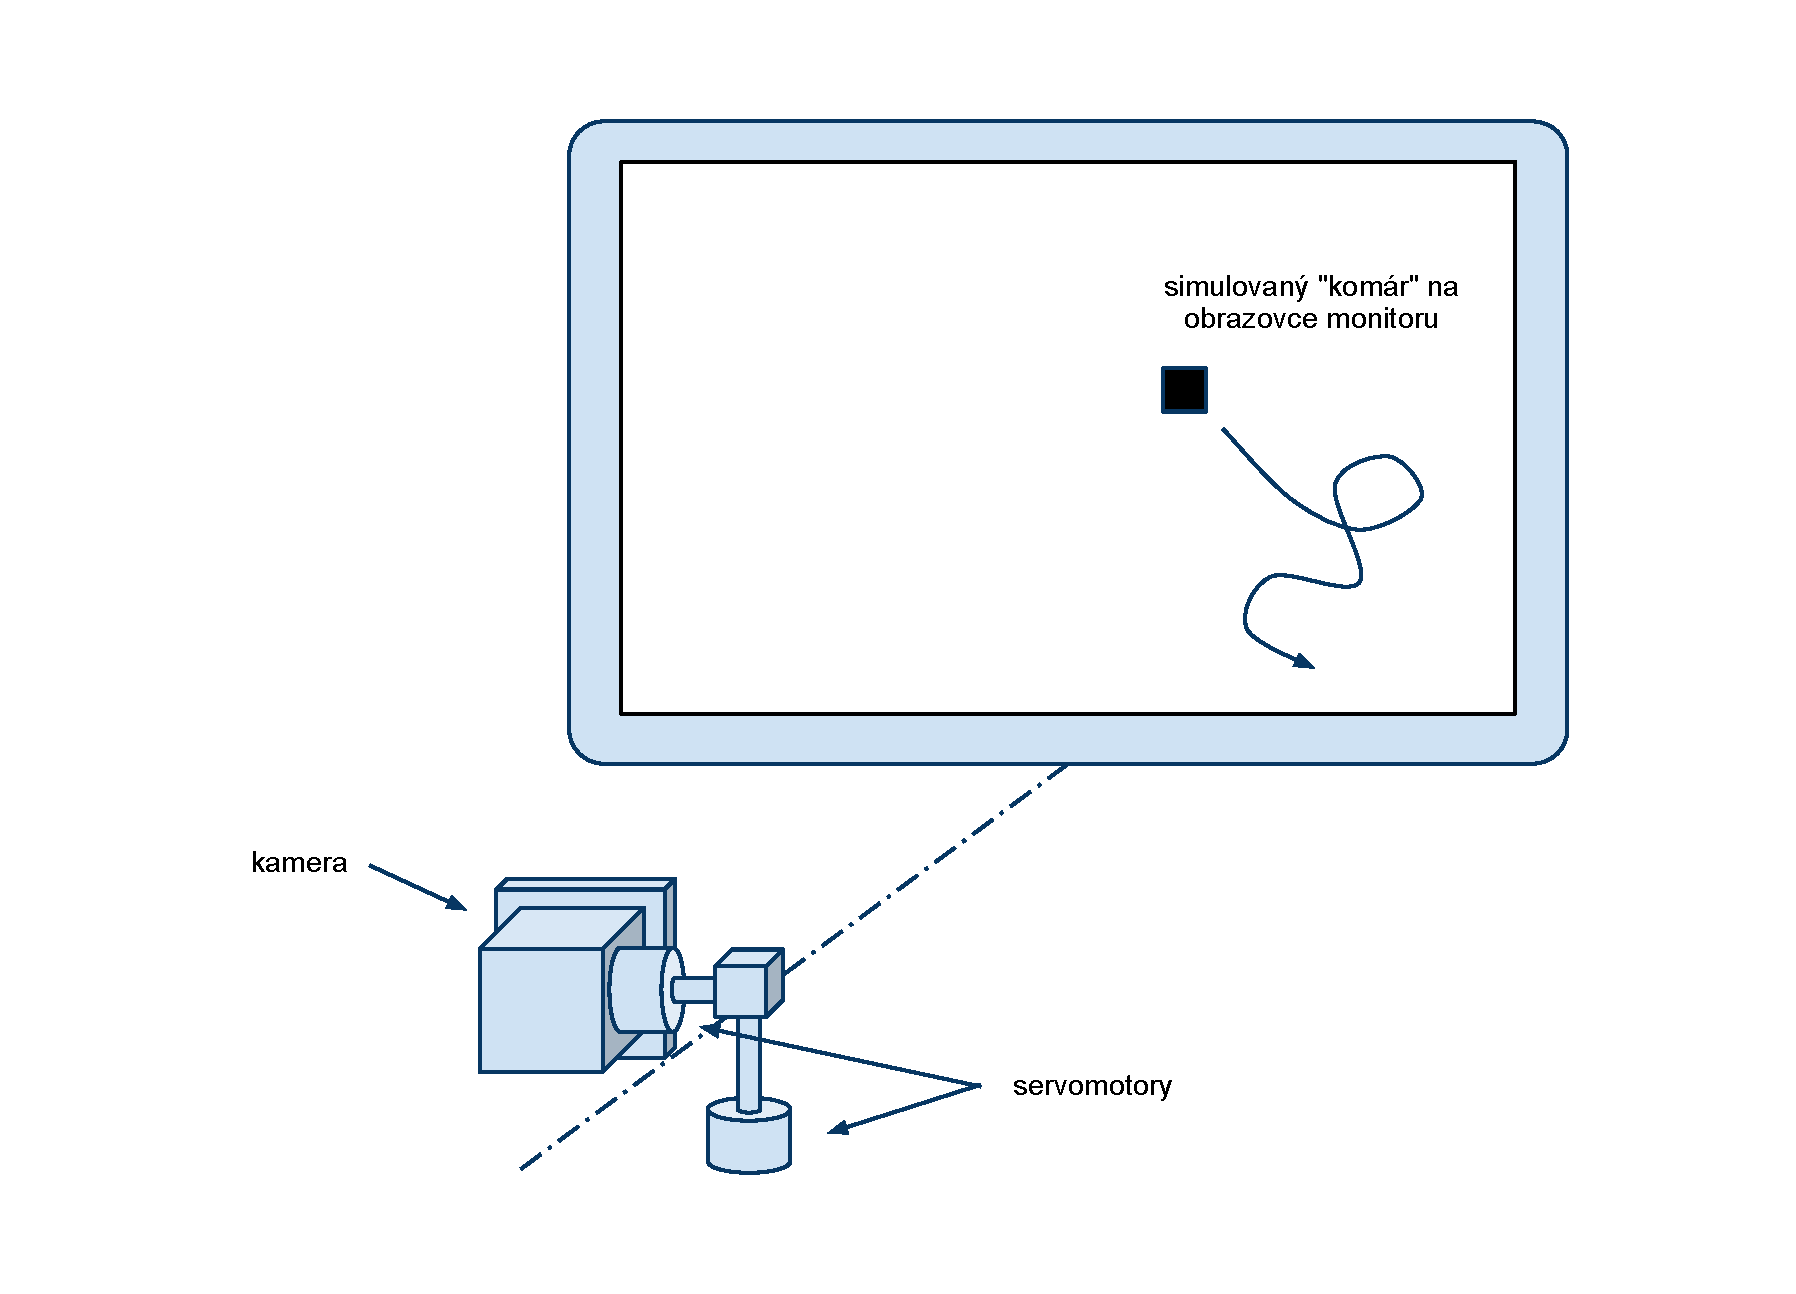
\includegraphics[width=1\columnwidth]{pics/usporadani_pracoviste}
			 \caption{Schematické znázornění uspořádání pracoviště „komár“}\label{fig:usporadaniPracoviste}
		\end{figure}

	\subsection{Popis pracoviště}

		Použité pracoviště „komár“ je tvořeno monitorem a kamerou umístěnou na „pan-tilt“ jednotce, která je namířena
		na monitor. Obrázek \ref{fig:usporadaniPracoviste} znázorňuje vzájemné uspořádání monitoru a kamery.
		Pan-tilt jednotka je tvořena dvěma mo\-de\-lář\-ský\-mi servy, která umožňují natáčení kamery okolo svislé osy
		(změnu azimutu, pan) a okolo vodorovné osy (změnu elevace, tilt).
		Podrobněji jsou parametry monitoru, kamery a jejich vzájemné konfigurace popsány v \cite{kamera}.
		Použita byla USB kamera Chameleon od firmy PointGrey \cite{kameraDatasheet} a na pan-tilt jednotce byly
		použity dva pohony AI-701 firmy Megarobotics řízené prostřednictvím sběrnice RS-232 \cite{servaManual}.

	\subsection{Použité softwarové prostředí}

		Řídicí program byl implementován v prostředí Matlab. Pro práci s kamerou (periodické vyčítání
		obrázků z kamery) byl použit Image Acquisition Toolbox \cite{imaq} a při zpracování obrázků
		byly použity morfologické funkce Image Processing Toolboxu \cite{imageProcessingToolbox}.

	\subsection{Ovládání servomechanismů}

		Pro řízení servomotorů bylo použito standardních funkcí Matlabu pro práci se sériovým rozhraním.
		Řídicí jednotce pohonů AI-701 je možné zasílat žádané absolutní úhly natočení jednotlivých serv
		v rozsahu 0-254, který odpovídá přibližně rozsahu 80 úhlových stupňů.

\section{Změny specifikace}

		%TODO: vymyslet to
		Díky použití pracovišťě číslo dva se neprojevila nelineární závislost otočení kamery na pozici komára. 
		Dále jsme pozorovali konstantní chování celé dynamické soustavy kamery se servy, tedy jsme ani neřešili 
		identifikaci soustavy.
		
\section{Řešení problému}

		\begin{figure}[!h]
			\centering
			 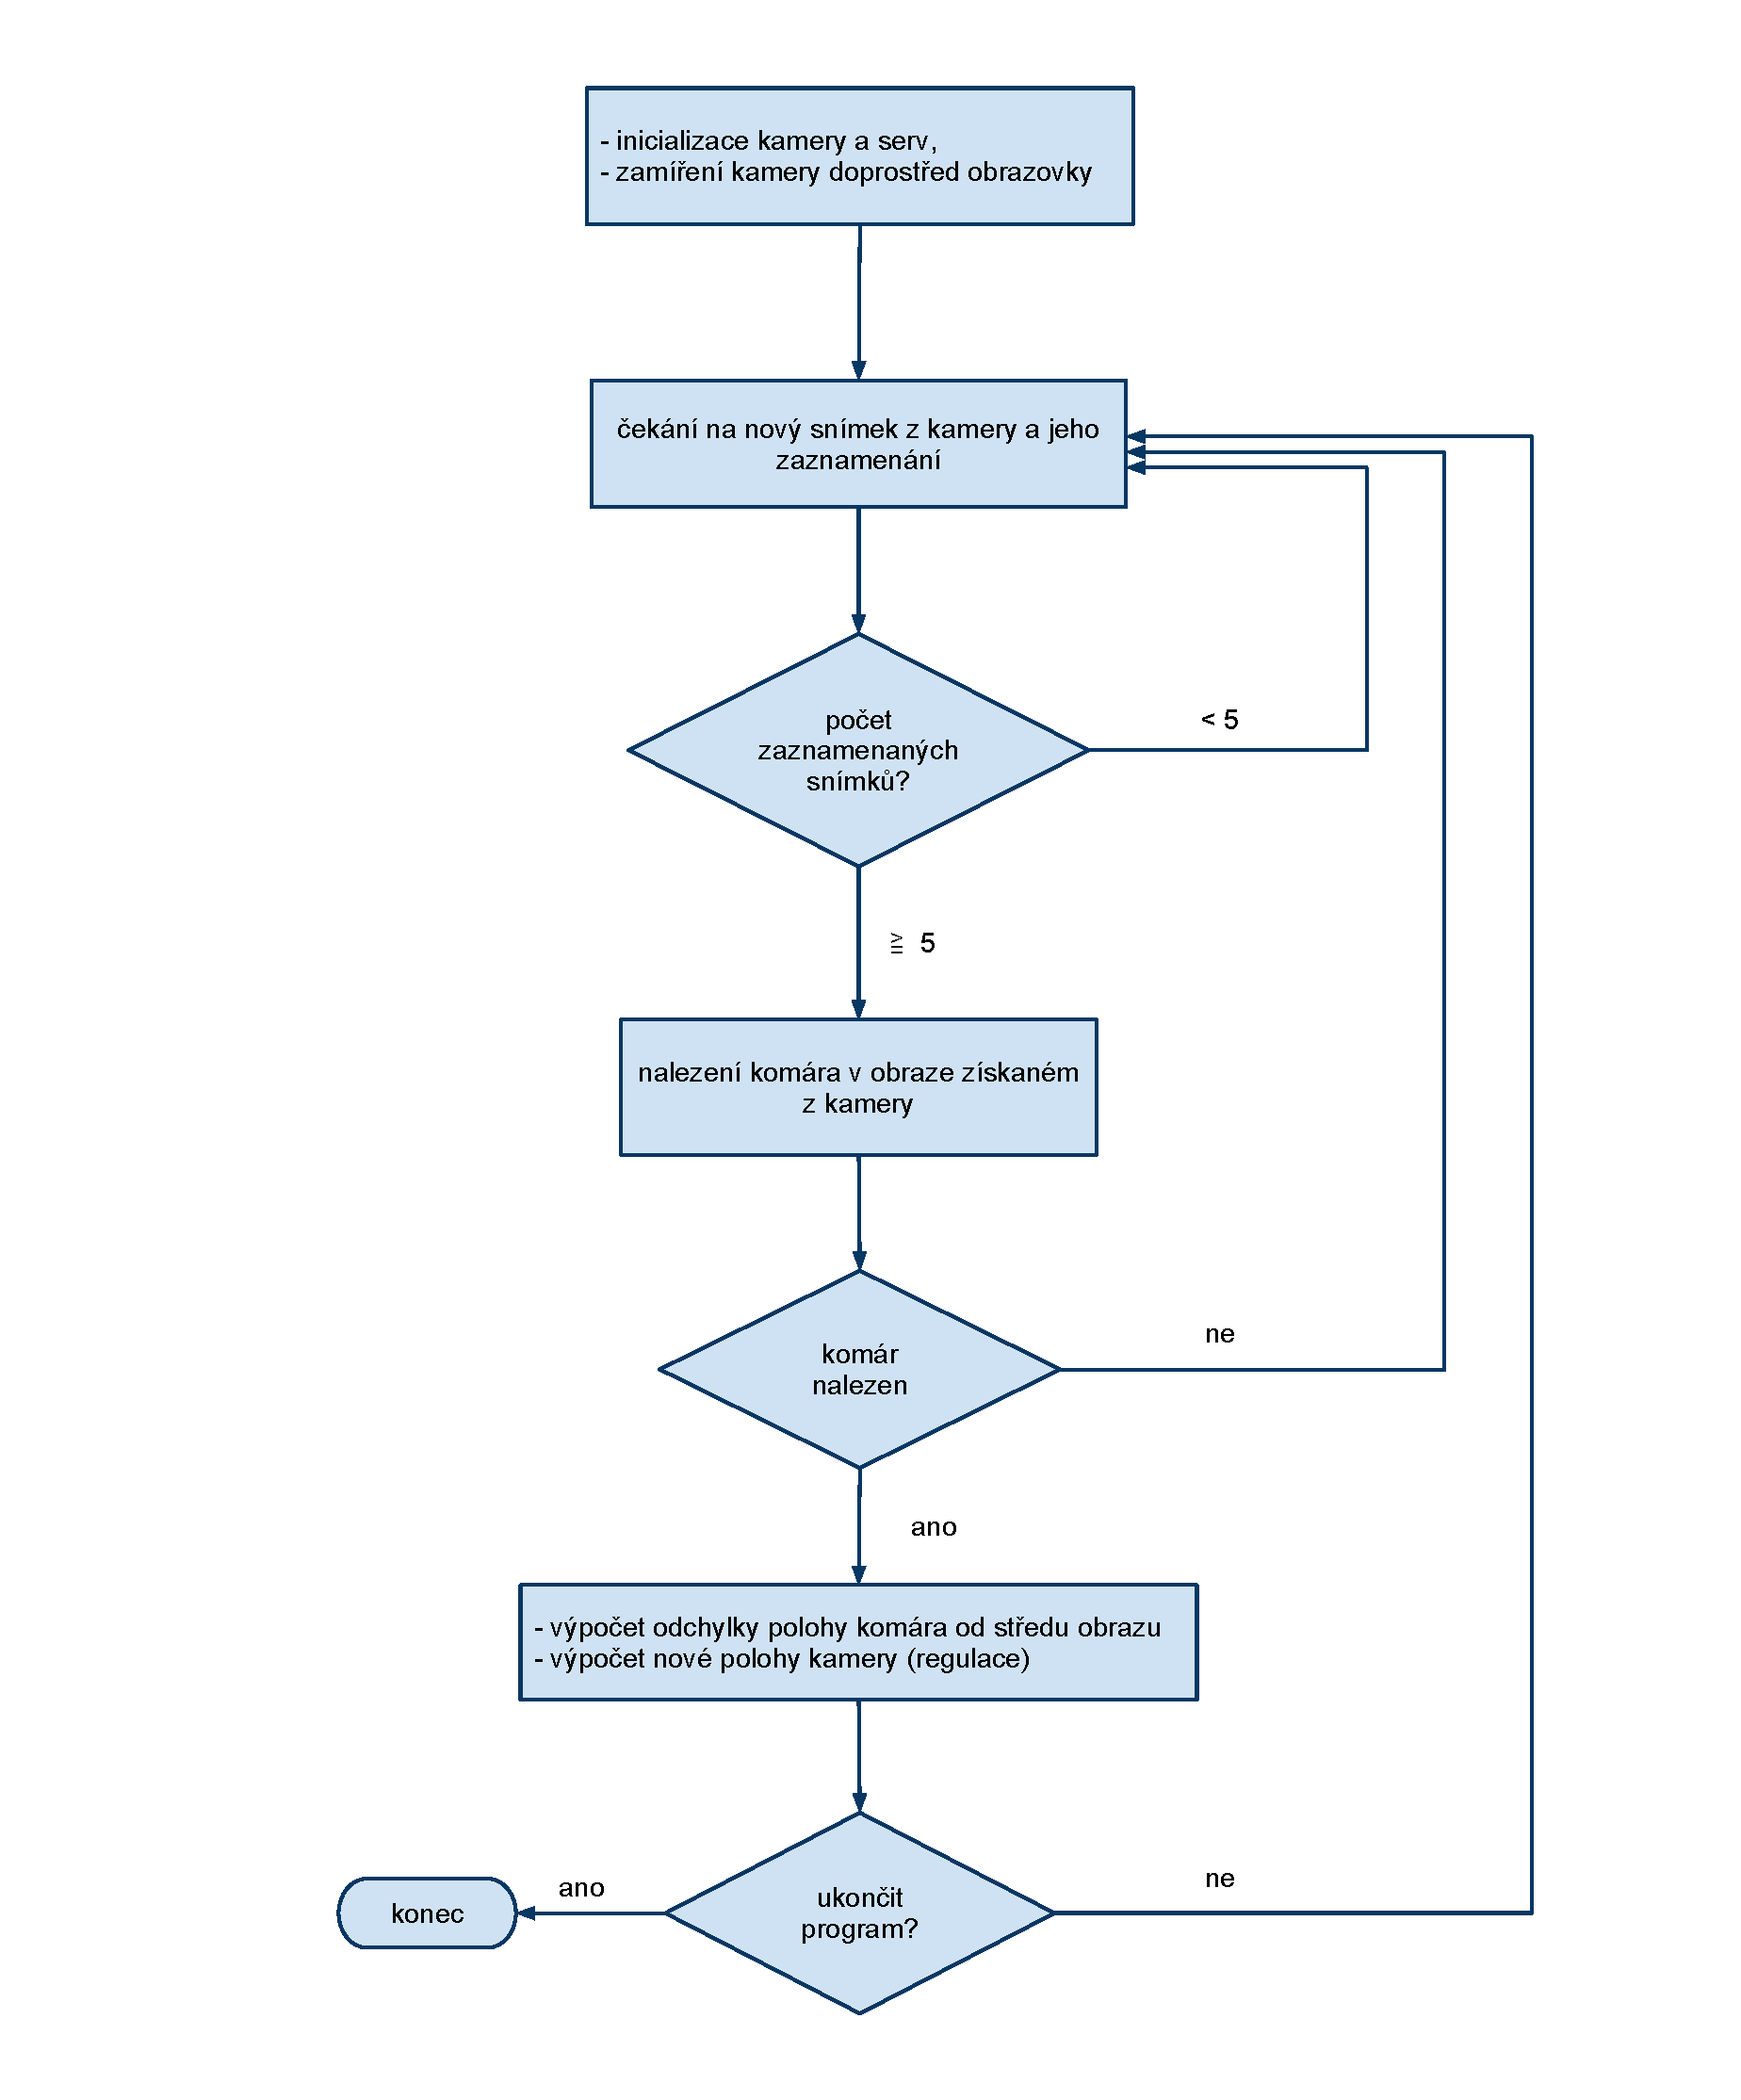
\includegraphics[width=1\columnwidth]{pics/vyvojovy_diagram_programu}
			 \caption{Vývojový diagram programu}\label{fig:Diagram_programu}
		\end{figure}

		Po spuštění programu se nejprve zincializují serva a kamera, 
		která se nastaví na střed obrazovky.
		Zde se vyčkává do příletu komára do zorného pole kamery.
		Jakmile se komár objeví v obraze, spustí se ukládání obrázků do pracovního prostoru, viz obr. \ref{fig:Diagram_programu}.

		Pro detekci komára v obraze se využívá znalosti řady omezení. 
		Nejprve se využívá barevné informace, komár je černý a pohybuje se na bílém pozadí.
		Ve vyčteném obrázku se tedy naleznou všechny tmavé oblasti. 
		Dále se využívá informace o maximálních rozměrech komára. 
		Je známo, že maximální velikost komára je $50$ pixelů. 
		Na základě této informace se zahodí všechny vybrané tmavé oblasti, 
		které jsou svou plochou či délkou hlavní osy větší než maximální komár.
		Ze zbylých oblastí je vybrána ta největší, která odpovídá komárovi.
		Je nalezen střed a tato informace se dále používá k regulaci kamerového systému.

\subsection{Implementace}

		Hlavní řídicí funkce se volá s využitím tzv. callback funkce, protože nám přišlo vhodné, 
		aby se perioda zpracování obrazu odvíjela od periody získávání obrázků.		
		K~regulaci se používá každý druhý obrázek a to z důvodů časové náročnosti regu\-lační smyčky.

		Ve vývojovém diagramu \ref{fig:Diagram_programu} lze pozorovat, že se zahazuje prvních pět obrázků.
		Pro toto opatření jsme se rozhodli proto, 
		že první obrázky bývají zarušeny chybou při vyčtení obrazu z kamery.

		Při zpracování obrazu a hledání komára používáme pouze zelenou složku,
		oproti debayerizaci je výpočetně nenáročná a 
		umožňuje v paměti uchovávat více obrázků. Pro zelenou složku jsme se rozhodli na základě pozorování, 
		jelikož poskytuje největší kontrast oproti ostatním barevným složkám.

		Takto upravený obraz je následně porovnán s~empiricky určeným prahem.
		Tím vznikne binární maska s~oblastmi, které vykazují barevnou podobnost s~hle\-da\-ným komárem, viz obr. \ref{fig:komar_obr2}.

		\begin{figure}[!htb]
			\subfloat[\label{fig:komar_obr1}]{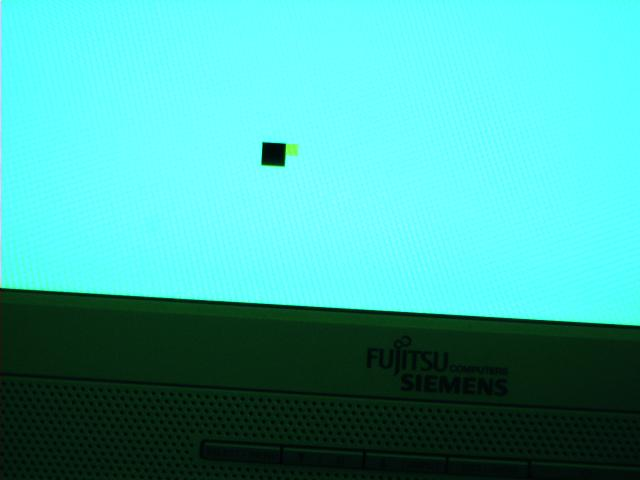
\includegraphics[width=0.49\columnwidth]{pics/zpracovani_obrazu-1}}
			\subfloat[\label{fig:komar_obr2}]{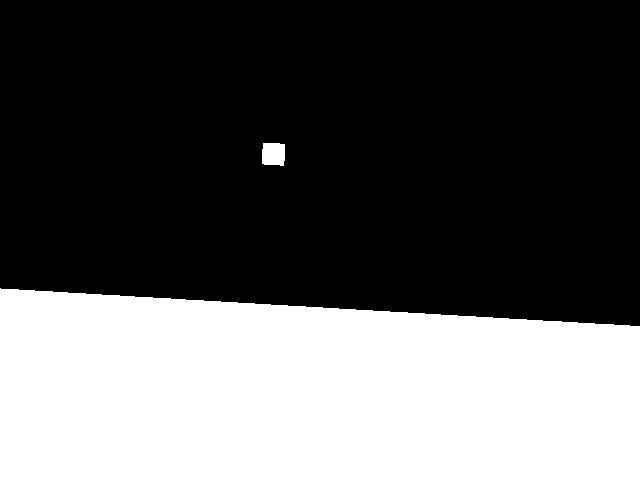
\includegraphics[width=0.49\columnwidth]{pics/zpracovani_obrazu-2}} \\
			\subfloat[\label{fig:komar_obr3}]{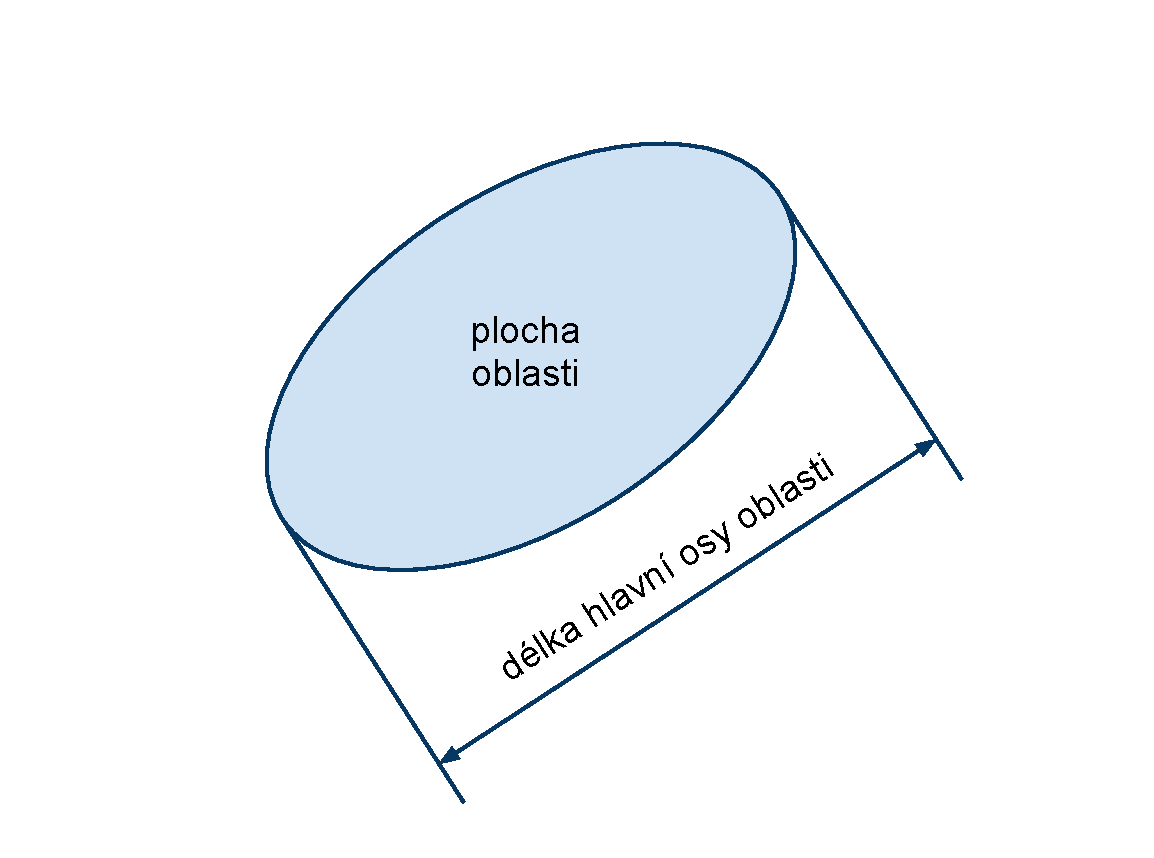
\includegraphics[width=0.49\columnwidth]{pics/delka_hlavni_osy_a_plocha_oblasti}}
			\subfloat[\label{fig:komar_obr4}]{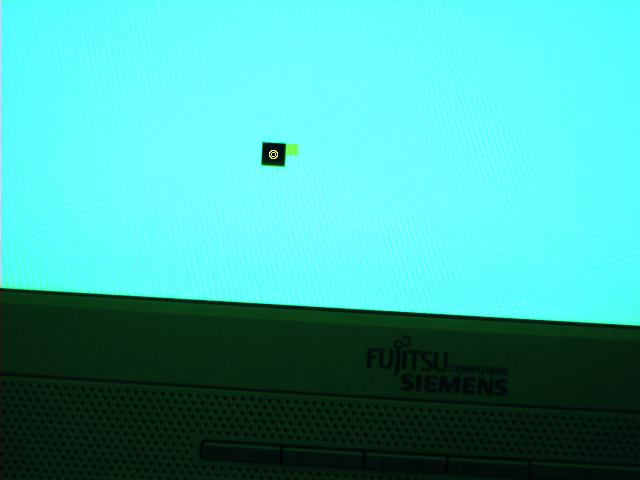
\includegraphics[width=0.49\columnwidth]{pics/zpracovani_obrazu-3}}
			%\caption{Zpracování obrazu pro nalezení polohy komára: \subref{fig:komar_obr1} obrázek sejmutý kamerou, \subref{fig:komar_obr2} obrázek po prahování, \subref{fig:komar_obr3} parametry nalezených oblastí, \subref{fig:komar_obr4} vyznačená poloha nalezeného komára}
			\caption{Zpracování obrazu pro nalezení polohy komára: (a) obrázek sejmutý kamerou, (b) obrázek po prahování, (c) parametry nalezených oblastí, (d) vyznačená poloha nalezeného komára}
		\end{figure}
		
		K~získání polohy komára v~obrazu byl použit jednoduchý algoritmus
		využíva\-jící morfologických funkci Matlabovského Image Processing Toolboxu. 
		V~binární masce jsou nalezeny souvislé oblasti.
		Dále jsou vyloučeny takové oblasti, 
		jejichž plocha a délka hlavní osy (obr. \ref{fig:komar_obr3}) jsou větší než maximální omezení komára.
		Ze zbývajících oblastí je vybrána ta, která má největší plochu. Pro tuto oblast je určena
		poloha středu v~pixelových souřadnicích, obr. \ref{fig:komar_obr4}.
		Z těchto hodnot se vypočte hodnota azimutu a elevace. 

	        Regulace, tedy výpočet nové polohy kamery $x_{new}, y_{new}$, je řešena jako PI
		regulátor. Vypočte se rozdíl mezi skutečnou a žádanou hodnotou $err$ a do
		proměné $sum_e$ se tato odchylka přičítá, při čemž její počáteční hodnota je
		nulová. Proměné $x, y$ jsou souřadnice aktuální polohy kamery.

		$$x_{new} = x + P\cdot err + I\cdot sum_e$$
		$$y_{new} = y + P\cdot err + I\cdot sum_e$$

		Pozice kamery je saturována na hodnoty, ve
		kterých je očekáván komár, tedy na hodnoty odpovídající kraji monitoru.

		Konstanty $P$ a $I$ jsou naladěny pro každý směr zvlášť.
		

%Funkce \textit{processNextFrame} tvoří zpětnovazební regulační smyčkou pro řízení polohy
%		kamery. Vstupem regulátoru je nejnovější získaný obrázek z~kamery a jeho
%		výstupem je nová poloha kamery.


%Před samotným výpočtem nové polohy kamery
%		je vyhodnocen nově zís\-ka\-ný obraz. Postup jeho zpracování je znázorněn na
%		obrázku~\ref{fig:zpracovaniObrazu}.  Nejprve je určena poloha komára v~obraze
%		(funkce \textit{findMosquitoInImage}) v~pixelových sou\-řad\-ni\-cích. Na základě odchylky
%		této polohy od středu obrázku potom funkce
%		\textit{mos\-quito\-Px\-PositionToAzimuthAndElevation} počítá odhad úhlů, o~které je
%		komár vy\-chý\-len od optické osy kamery. Pro urychlení celé smyčky jsou data pouze
%		ukládána, nikoliv zobrazována. Uživatel si snadno tato data přehraje offline.

\section{Experimentální výsledky}

\subsection{PI regulátor}

Na základě pozorování jsme rozdělili regulátor polohy na regulaci v každé ose zvlášť.
Pro testování jsme si zobrazovali graf pozice komára v jedné ose a pozorovali vliv konstant na kmitání kolem žádané polohy. 
Pro oba směry jsme naladili konstanty tak, abychom získali, co nejlepšího sledování komára.
Pro osu $y$ se nám podařilo získat uspokojivý výsledek, viz \ref{fig:osay}. 

\begin{figure}[!h]
	\centering
	%\includegraphics[width=1\columnwidth]{pics/}
	\caption{Pozice komára v ose y a průběh integrační sumy}\label{fig:osay}
\end{figure}

Bohužel musíme konstatovat, že podobně uspokojivého výsledku se nám nepodařilo dosáhnout pro osu $x$. 
Po příletu komára k okraji monitoru a následném odletu se zvětšila odchylka skutečné od žádané polohy 
a regulátor se značně rozkmital. 

Tato situace vedla k tomu upravit parametry regulátoru, což vedlo k zhoršení sledování komára při malých odchylkách, 
tedy při letu uprostřed obrazovky. Regulátor jsme tedy naladili jako kompromis mezi pozorovanými stavy. 

\begin{figure}[!h]
	\centering
	%\includegraphics[width=1\columnwidth]{pics/}
	\caption{Pozice komára v ose x a průběh integrační sumy}\label{fig:osax}
\end{figure}

\subsection{Predikce letu komára}

Model komára zachovává fyzikální podstatu letu, zrychluje a zpomaluje s koneč\-ným zrychlením a nemění razantně směr.
Lze tedy předpokládat, že pohyb komára na obraze je generován určitou funkcí a 
nová pozice komára lze vypočítat jako taylorův polynom. 
Rozhodli jsme se pro odhadování nové pozice komára z posledních pěti naměřených hodnot.
Tuto hodnotu jsme zvolili jako optimum mezi dosažitelnou přesností a časovou náročností výpočtu.

Experimenty poukázaly na dva problémy s tímto základním přístupem. 
Za prvé jsme došli k závěru, že pohyb komára je zatížen náhodným prvkem, který zhoršuje možnosti predikce pohybu.
Za druhé měla predikce vliv na chování soustavy pouze tehdy, pokud se použil samotný P regulátor. 
S využitím PI regulátoru predikce nepřinášela žádné významné zlepšení chování systému.


\section{Diskuze a Závěr}

S využitím callback funkce a 
morfologických funkcí Image Processing Toolboxu jsme dosáhli toho, že zpracování a 
detekce komára v obraze trvá v průměru pouhých $0,08 s$. 
Minimální perioda s~jakou je možné získat obrázky z~kamery je $0,067 s$,
proto se pro regulaci kamery používá každý druhý obrázek.

Pokud bychom měli na úlohu více času, rádi bychom se zaměřili na predikci pohybu komára jiným přístupem.
Věříme, že by nám pomohla vyřešit problém s PI regulátorem.
K další přístupům predikce patří například Kalmanův filtr, 
ale v tomto přístupu očekáváme problémy s linearitou. 
 
\section*{Doporučení pro další cvičení}

Úloha se nám z počátku velmi líbila, především proto, že se jednalo o otevřený problém. 
Bylo čistě na studentovi, jak daný problém vyřeší. 
V průběhu semestru se ovšem projevilo, že původní výhoda se stala spíše nevýhodou. 
K úloze na cvičení člověk používal pouze znalosti získané dříve a ztrácel kontakt s probíranou látkou na přednáškách.
Myslíme, že by bylo lepší ponechat otevřenost problému, ale více ho provázat s problematikou přednášek.

Dále jsme ocenili rezervační systém, ale dvě stanovišťě se ukázala býti nedostačující. 
Možná by do příště pomohlo, kdyby byla dána k dispozici série testovacích dat. 
Student by pak mohl pracovat více „offline“ a především v počátku semestru, 
kdy úloha nefungovala, by se studentovi umožnilo na úloze více pracovat.
Myslíme, že by bylo dobré vyžadovat v první polovině semestru více práce, 
v tomto období je ještě relativně čas. 
Naopak v druhé polovině je student vytížen dalšími projekty.



\bibliographystyle{splncs03}
\bibliography{report}

\end{document}
 
